\chapter{Comparison of Different Algorithms}

% Do a good job of explain PSNR via this paper: https://en.wikipedia.org/wiki/Peak_signal-to-noise_ratio

We compare the performance of the different algorithms used throughout this report. We also test the performance of the forward method and backward method on different pinhole sizes (3x3 pinhole vs 5x5 pinhole). Potential advantages of the 3x3 pinhole include improved resolution. However, the 3x3 pinhole filters out less light than the 5x5 pinhole, which can lead to more blurring.  

\begin{figure}
    \centering
    \textbf{3x3 Forward Algorithm}\par\medskip
    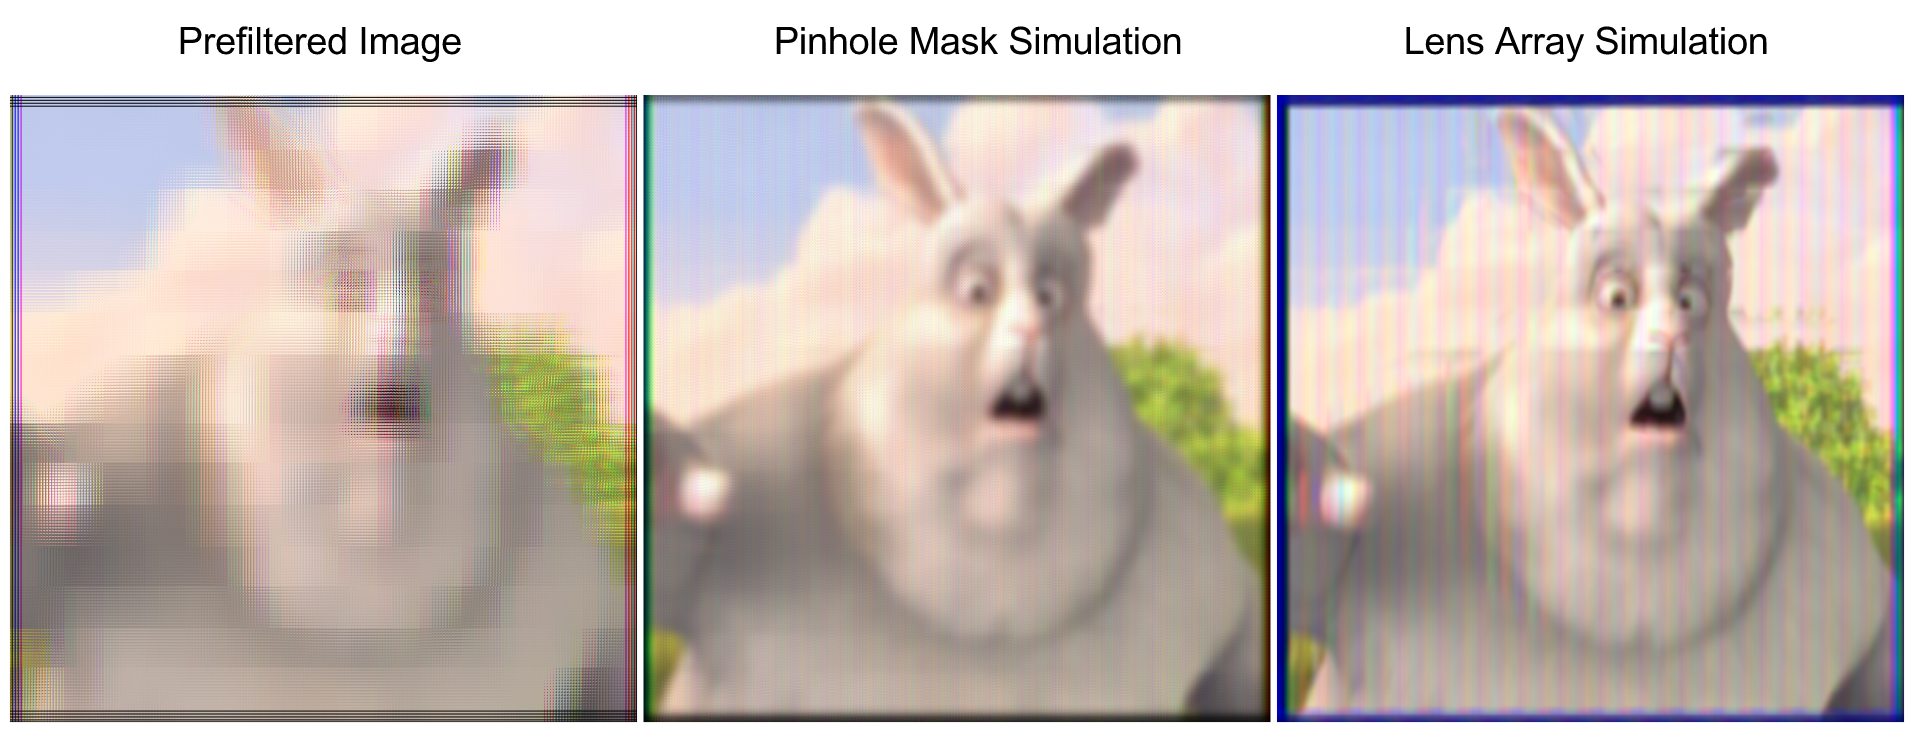
\includegraphics[width=\columnwidth]{chapters/chapter9/images/3x3_forward.png}
\end{figure}

\begin{figure}
    \centering
    \textbf{5x5 Forward Algorithm}\par\medskip
    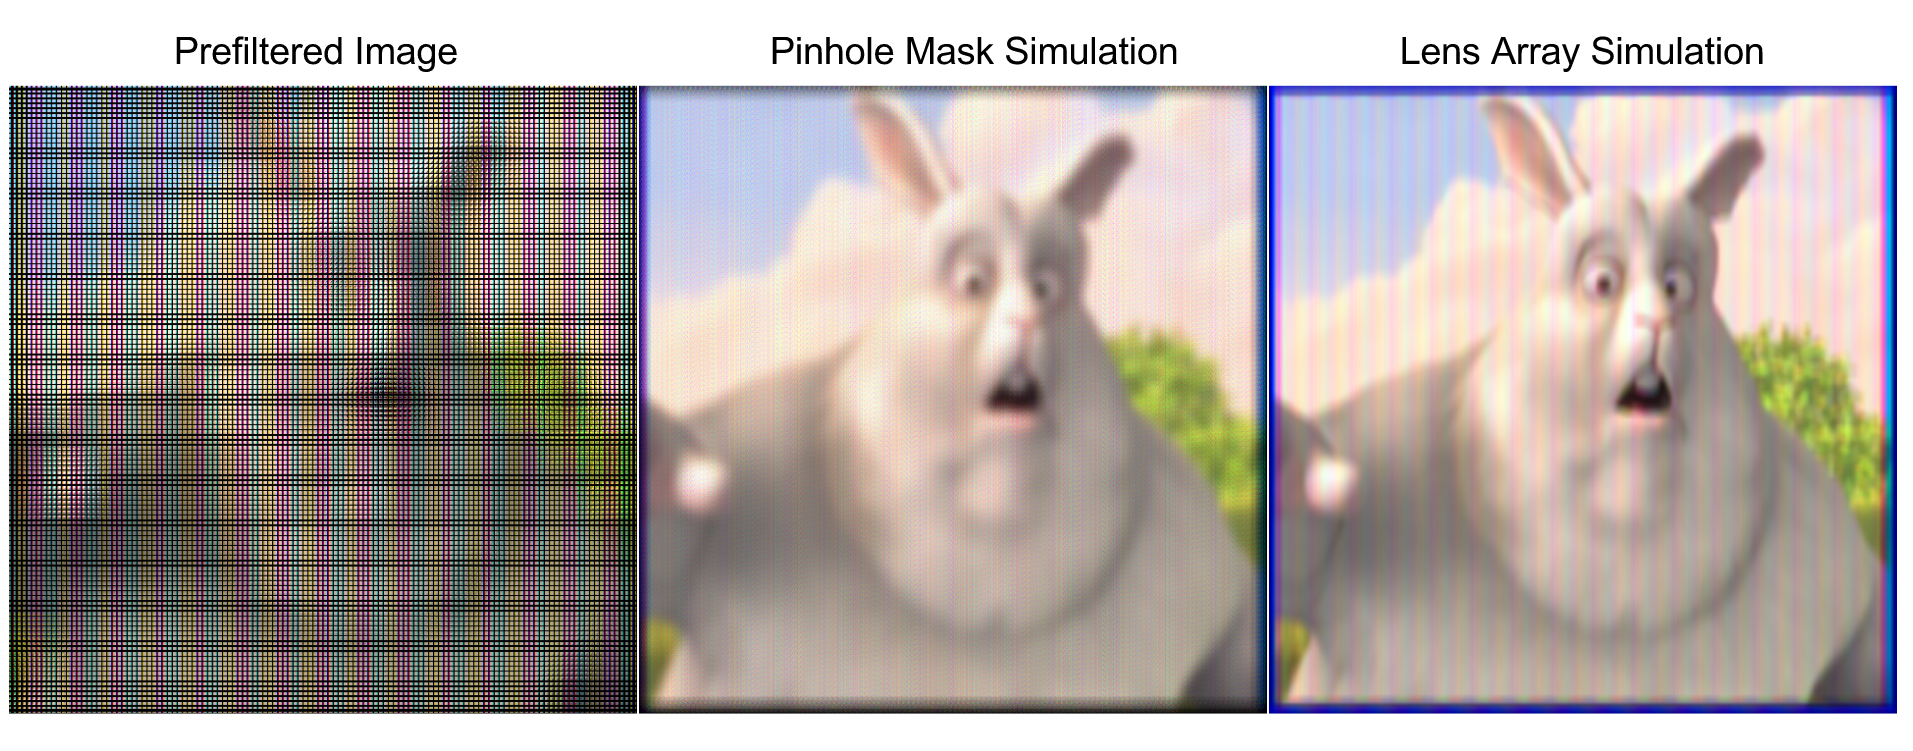
\includegraphics[width=\columnwidth]{chapters/chapter9/images/5x5_forward.png}
\end{figure}

\begin{figure}
    \centering
    \textbf{3x3 Backward Algorithm}\par\medskip
    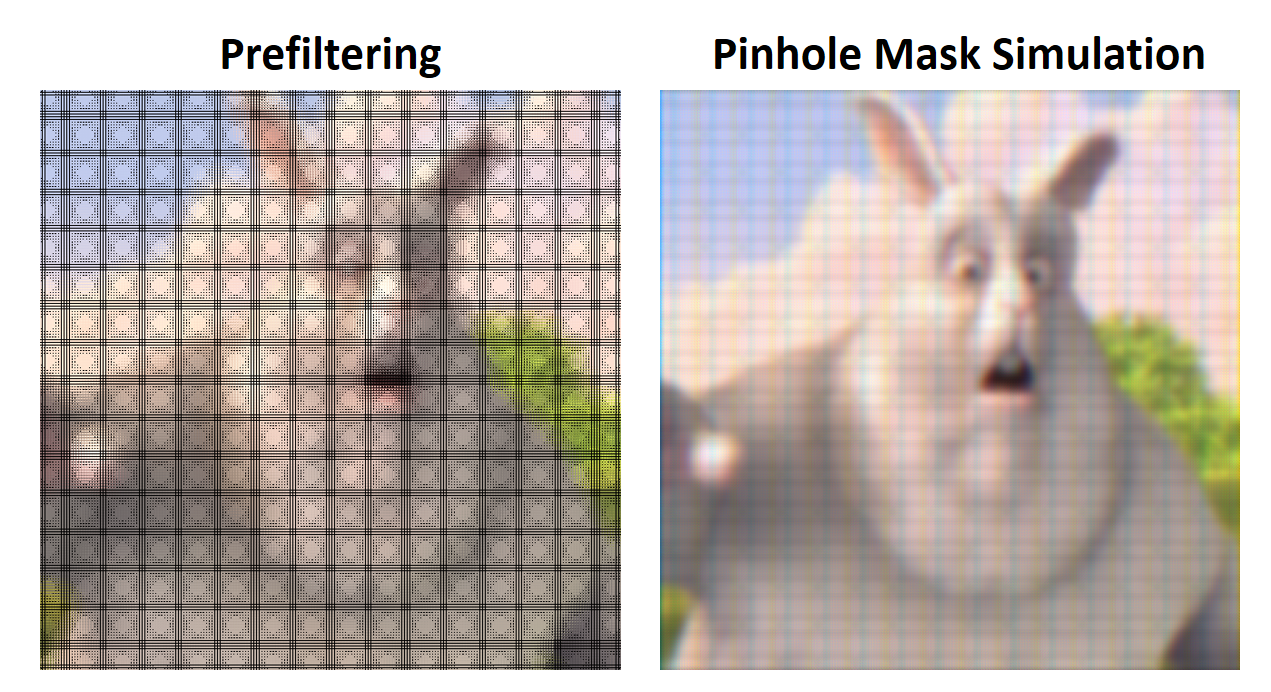
\includegraphics[width=\columnwidth]{chapters/chapter9/images/3x3_backward.png}
\end{figure}

\begin{figure}
    \centering
    \textbf{5x5 Backward Algorithm}\par\medskip
    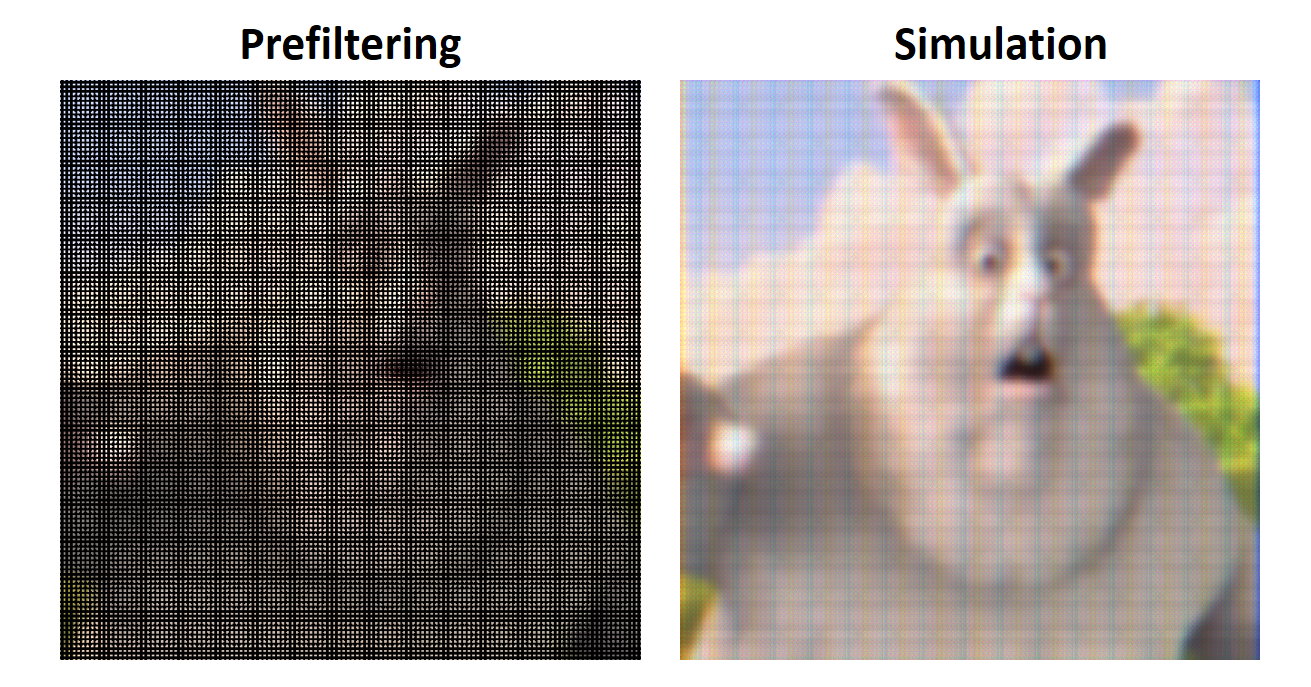
\includegraphics[width=\columnwidth]{chapters/chapter9/images/5x5_backward.png}
\end{figure}

\begin{figure}
    \centering
    \textbf{Huang's Algorithm at One Angle}\par\medskip
    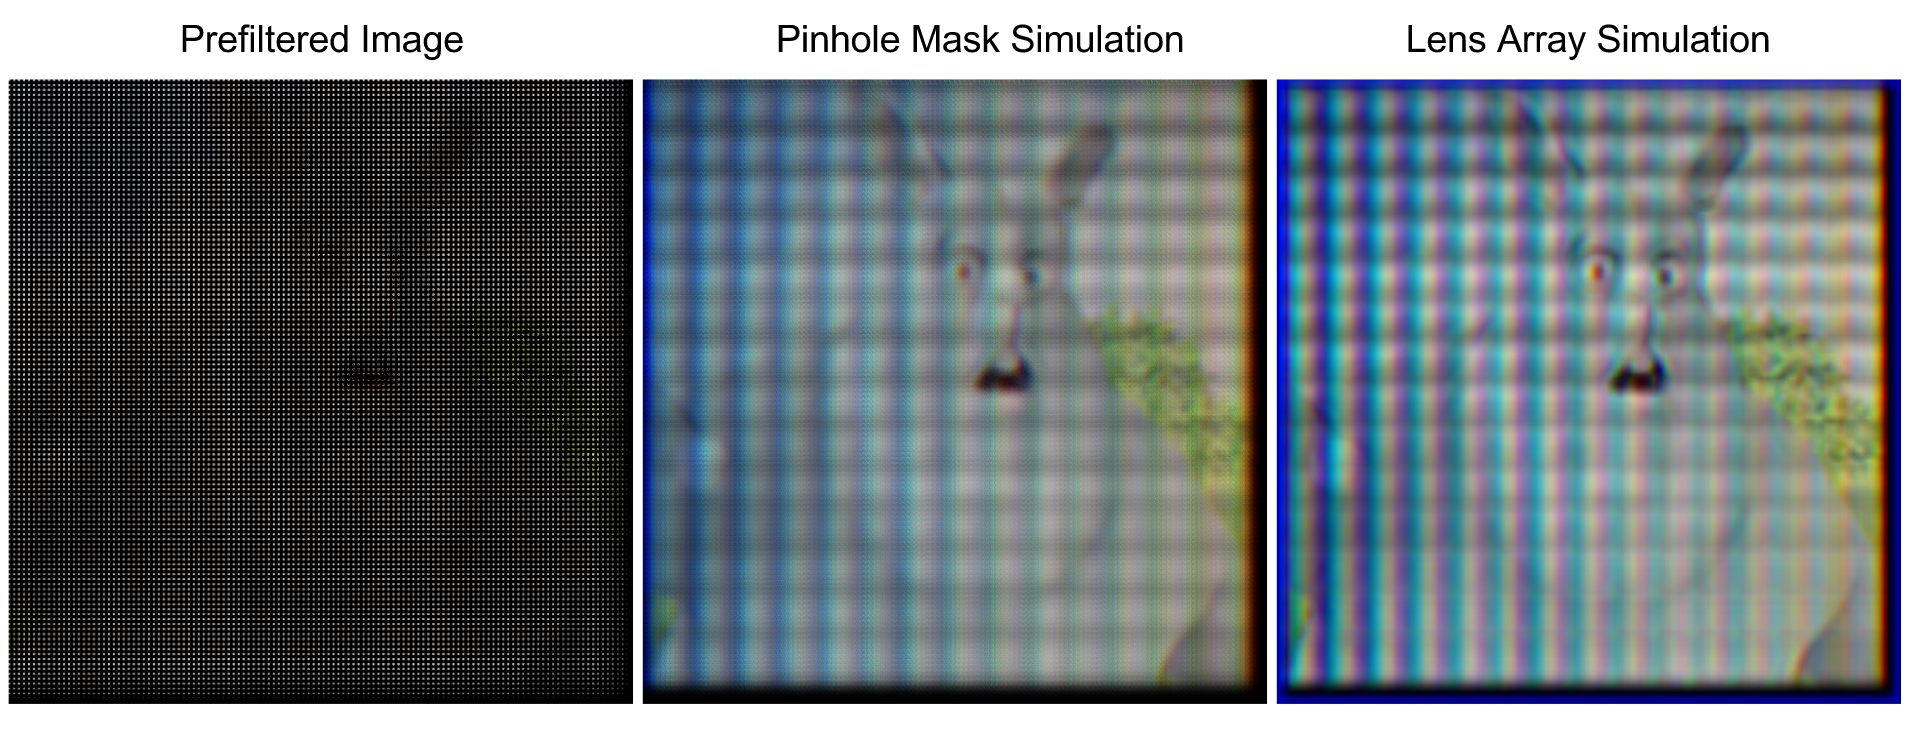
\includegraphics[width=\columnwidth]{chapters/chapter9/images/Huang_1_angle.png}
\end{figure}

\begin{figure}
    \centering
    \textbf{Huang's Algorithm at All Angles}\par\medskip
    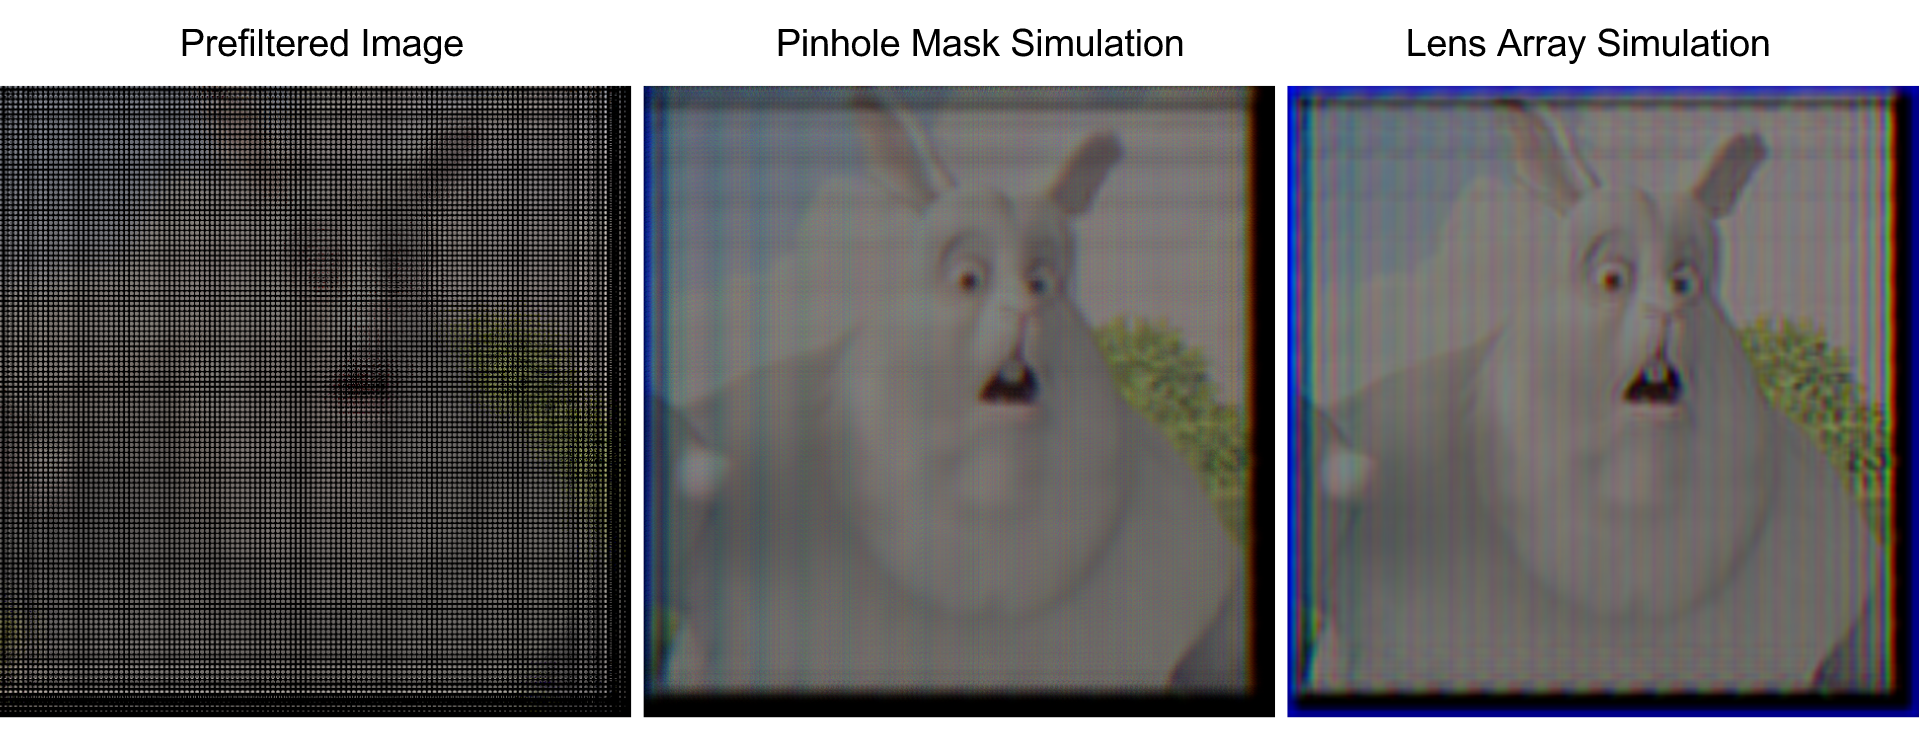
\includegraphics[width=6in]{chapters/chapter9/images/Huang_all_angle.png}
\end{figure}

\begin{figure}
    \centering
    \textbf{RMSE}\par\medskip
    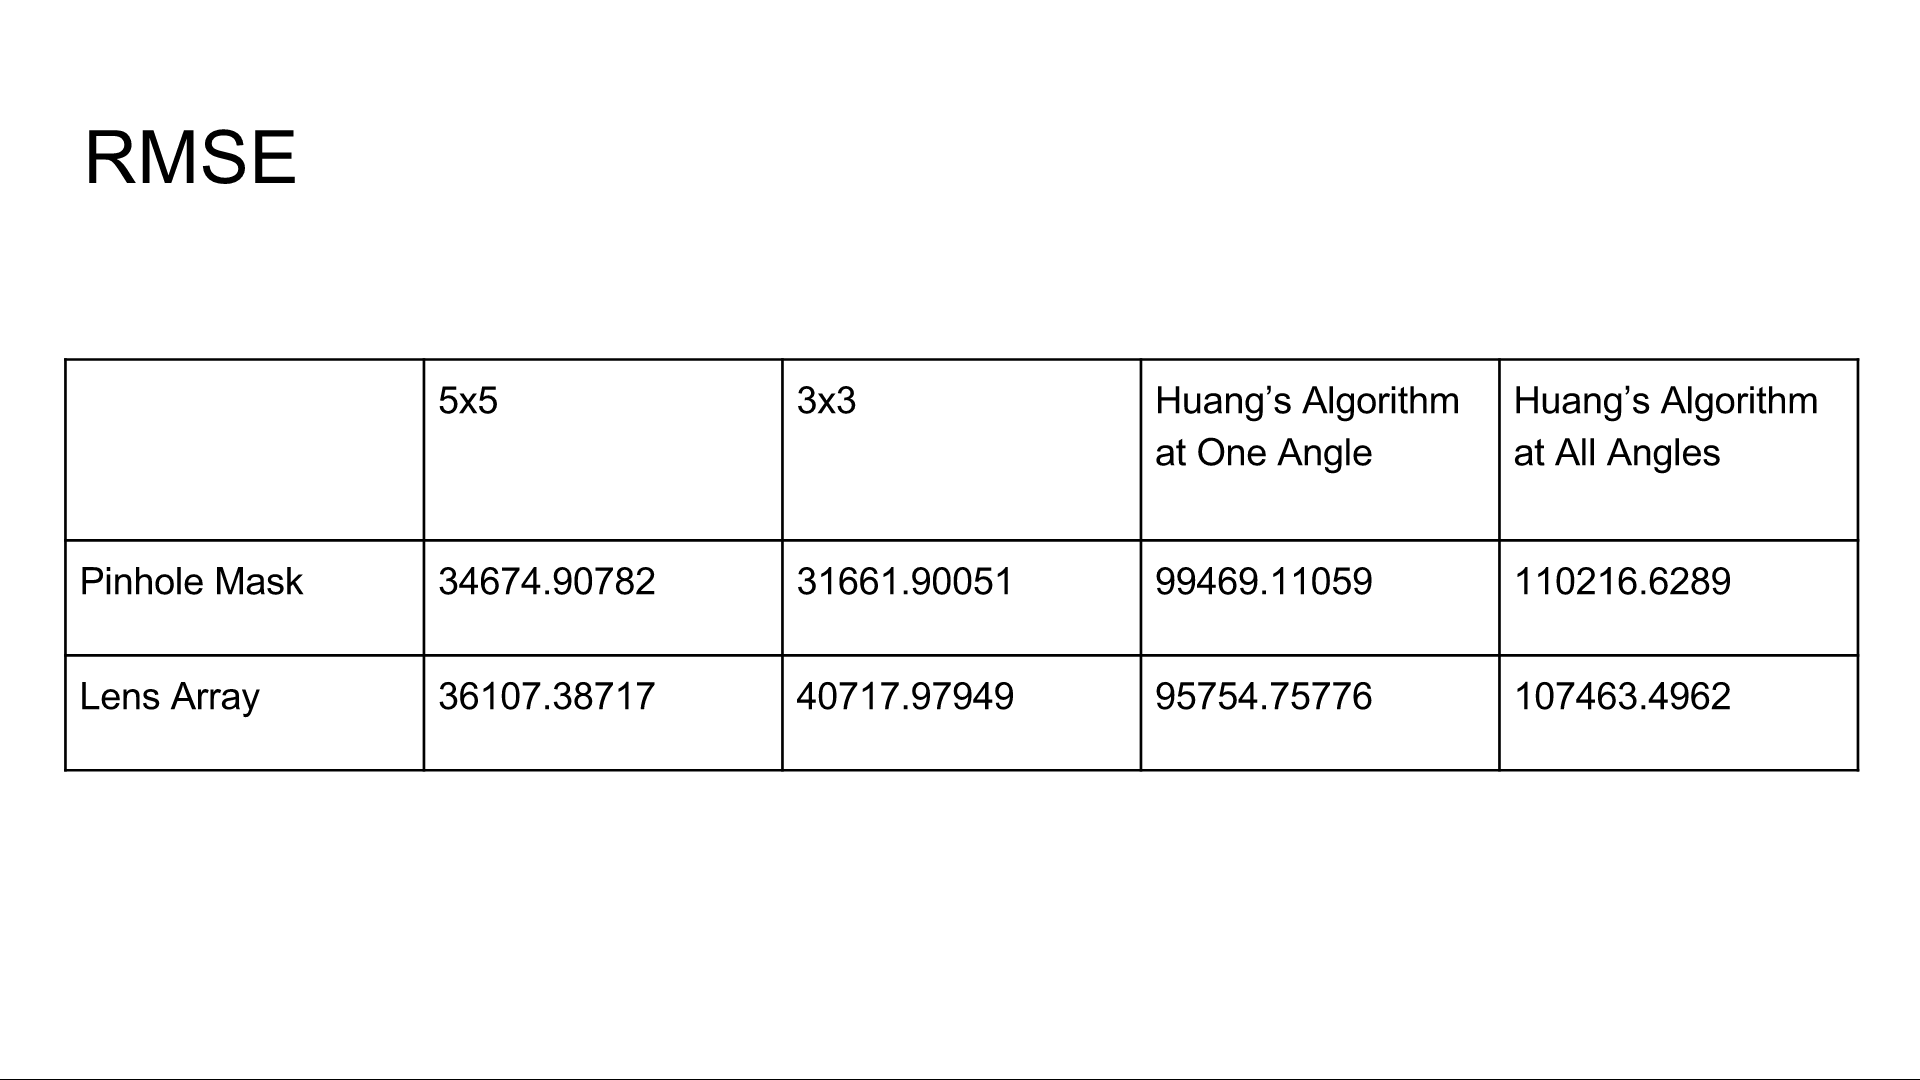
\includegraphics[width=6in]{chapters/chapter9/images/RMSE.png}
\end{figure}

\begin{figure}
    \centering
    \textbf{PSNR (Peak Signal to Noise Ratio)}\par\medskip
    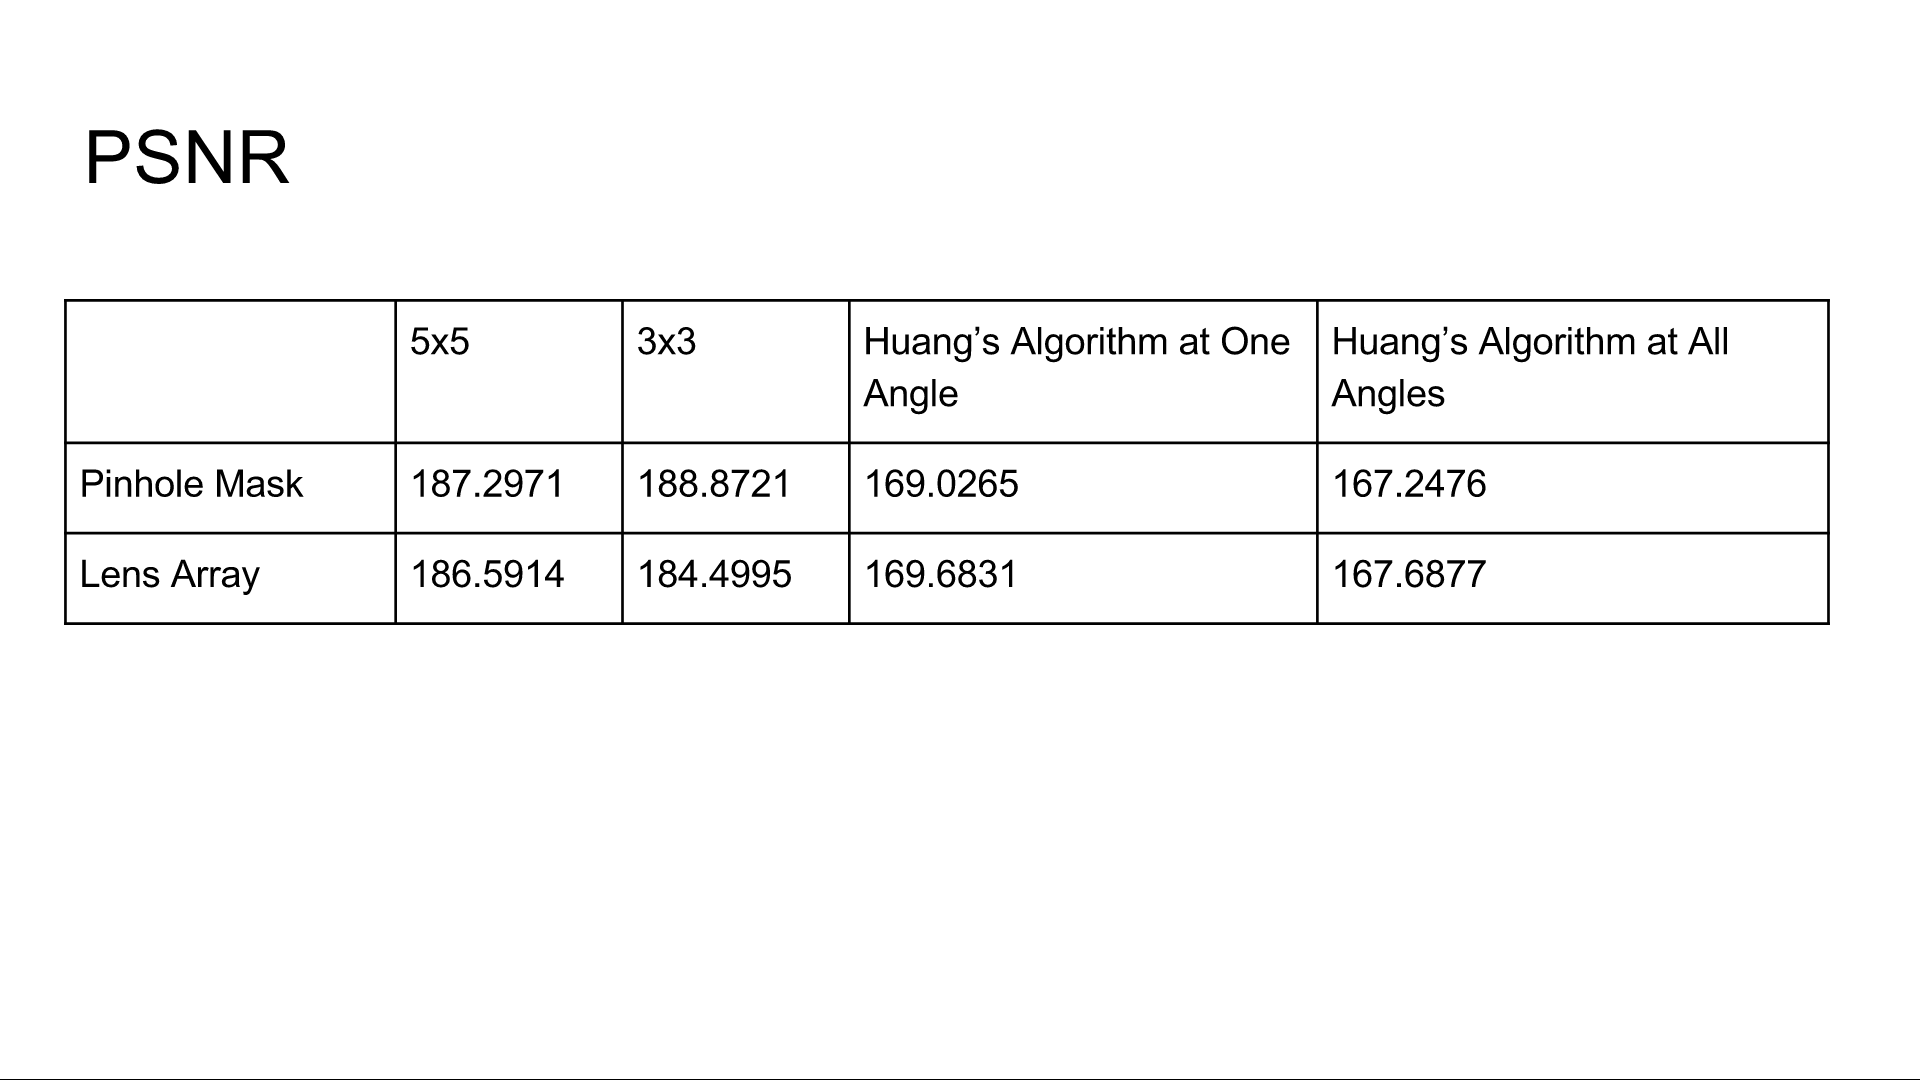
\includegraphics[width=6in]{chapters/chapter9/images/PSNR.png}
\end{figure}

\begin{figure}
    \centering
    \textbf{Contrast Loss}\par\medskip
    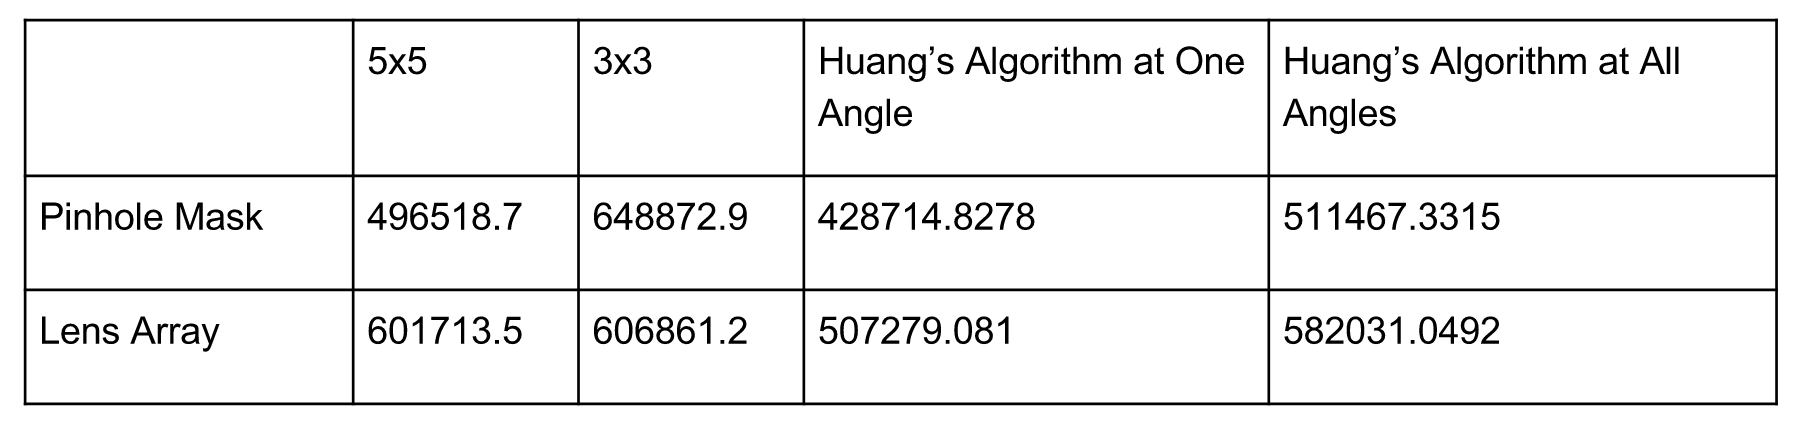
\includegraphics[width=\columnwidth]{chapters/chapter9/images/Contrast_Loss.png}
\end{figure}
